\documentclass{article}
\usepackage[utf8]{inputenc}
\usepackage{titling}
\usepackage{graphicx}
\usepackage{xcolor}
\usepackage[colorlinks=true,linkcolor=darkgray, urlcolor =gray]{hyperref}
\usepackage[spanish]{babel}
\DeclareUnicodeCharacter{301}{~}
\usepackage{url}
\DeclareUnicodeCharacter{202F}{\,}


\title{Programación Bluetooth en Java}
\author{Cristina Díaz García}
\date{Noviembre 2018}

\renewcommand\maketitlehooka{\null\mbox{}\vfill}
\renewcommand\maketitlehookd{\vfill\null}


\begin{document}

\addcontentsline{toc}{section}{Índice general}

\begin{titlingpage}
\maketitle

\begin{center}
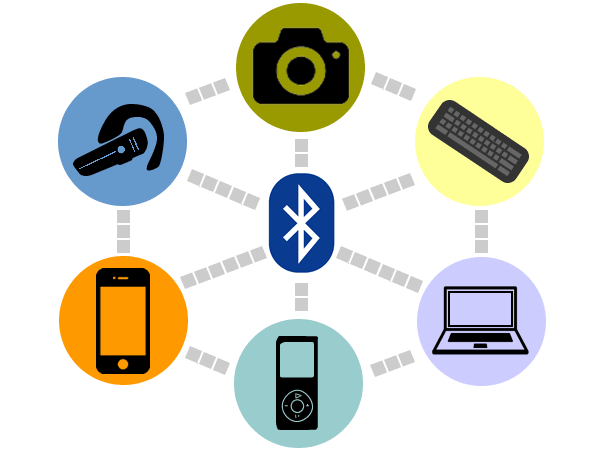
\includegraphics[scale=0.5]{imagenes/Bluetooth.png} 
\end{center}

\end{titlingpage}

\newpage

\tableofcontents

\newpage

\section{DISPOSITIVO DE COMUNICACIÓN BLUETOOTH}

\subsection{Ex1LocalInfo.java}

Usando los métodos \textit{getLocalDevice} y \textit{getProperty} de la clase LocalDevice obtenemos una clase LocaDevice y las propiedades, respectivamente. Usando los métodos \textit{getBluetoothAddress} y \textit{getFriendlyName} mostramos la dirección bluetooth y el nombre (\textit{friendly name}).

\begin{flushleft}
	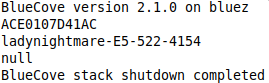
\includegraphics[scale=0.75]{imagenes/Ex1LocalInfo.png} 
\end{flushleft}

\section{DESCUBRIMIENTO DE DISPOSITIVOS REMOTOS}

\subsection{Ex2DiscoverNearDevices.java}

Haciendo uso de un \textit{listener}, hacemos una búsqueda de los dispositivos bluetooth visibles de alrededor, los guardamos en un vector e imprimimos su dirección bluetooh, y si fuera posible, su \textit{friendly name}.

\begin{flushleft}
	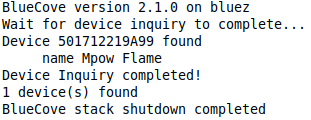
\includegraphics[scale=0.6]{imagenes/Ex2DiscoverNearDevices.png} 
\end{flushleft}

\subsection{Ex3DiscoverKnownDevice.java}

Haciendo uso de un \textit{listener}, hacemos una búsqueda de los dispositivos bluetooth restringiéndola, ya sea a una dirección bluetooth o a un \textit{friendly name} concretos, los guardamos en un vector si los encontraramos e imprimimos su dirección bluetooh, y si fuera posible, su \textit{friendly name}.

\begin{flushleft}
	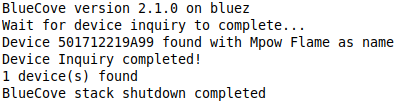
\includegraphics[scale=0.6]{imagenes/Ex3DiscoverKnownDevice.png} 
\end{flushleft}

\section{DESCUBRIMIENTO DE SERVICIOS}

\subsection{Ex4ServicesKnownDevice.java}

Primero hacemos una llamada a la clase \textit{Ex3DiscoverKnownDevice.java} previamente creada, para así encontrar solo el dispositivo deseado, y entonces guardamos su dirección bluetooh, para después, usando el método \textit{searchServices} de la clase \textit{DiscoveryAgent} buscar los servicios del dispositivo que habíamos guardado.

\begin{flushleft}
	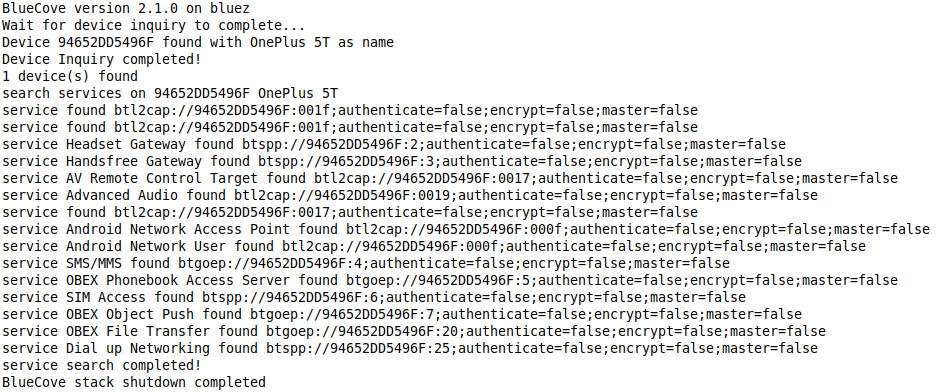
\includegraphics[scale=0.5]{imagenes/Ex4ServicesKnownDevice.png} 
\end{flushleft}

\subsection{Ex5ServicesNearDevices.java}

Primero hacemos una llamada a la clase \textit{Ex2DiscoverNearDevices.java} previamente creada, para así encontrar todos los dispositivos cercanos, y entonces guardamos sus direcciones bluetooh, para después, usando el método \textit{searchServices} de la clase \textit{DiscoveryAgent} recorrer el vector en el que habíamos guardado las direcciones buscando los servicios.

\begin{flushleft}
	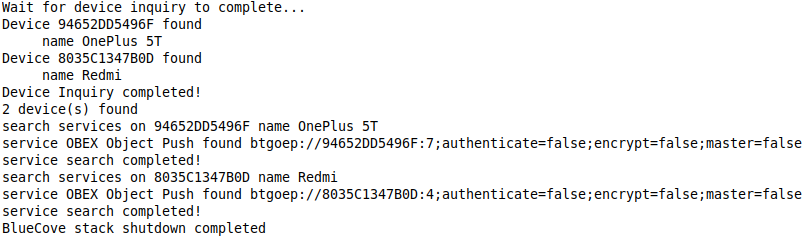
\includegraphics[scale=0.5]{imagenes/Ex5ServicesNearDevices.png} 
\end{flushleft}

\subsection{Ex6PublicServicesNearDevices.java}

Primero hacemos una llamada a la clase \textit{Ex2DiscoverNearDevices.java} previamente creada, para así encontrar todos los dispositivos cercanos, y entonces guardamos sus direcciones bluetooh, para después, usando el método \textit{searchServices} de la clase \textit{DiscoveryAgent} recorrer el vector en el que habíamos guardado las direcciones buscando los servicios públicos.

\begin{flushleft}
	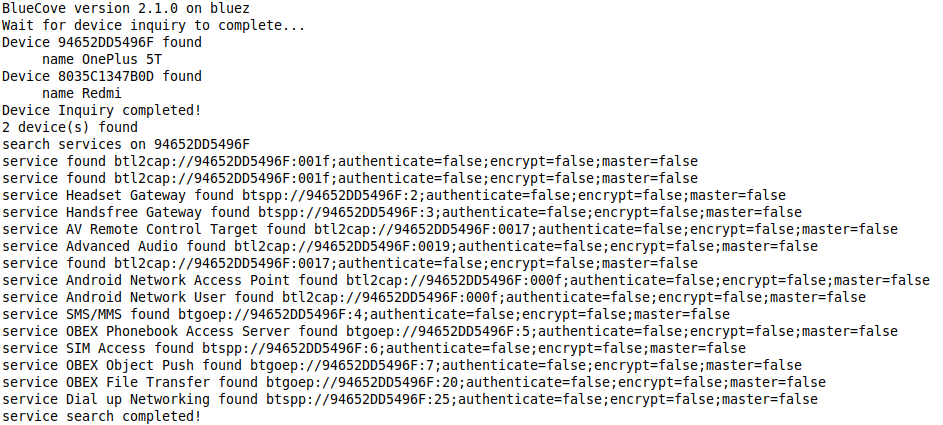
\includegraphics[scale=0.5]{imagenes/Ex6PublicServicesNearDevices_1.png} 
	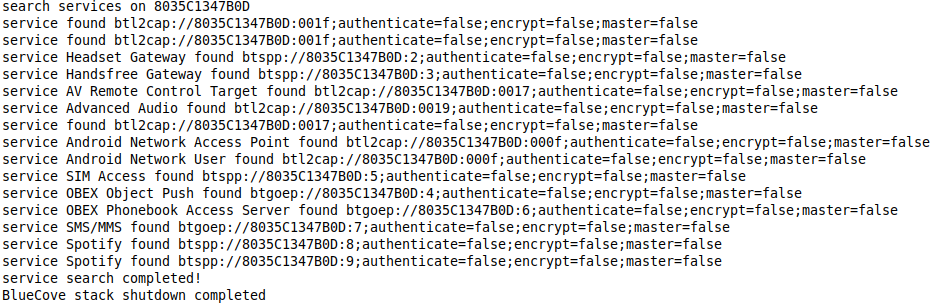
\includegraphics[scale=0.5]{imagenes/Ex6PublicServicesNearDevices_2.png} 
\end{flushleft}

\subsection{Ex7DeviceAndService.java}

Primero hacemos una llamada a la clase \textit{Ex3DiscoverKnownDevice.java} previamente creada, para así encontrar solo el dispositivo deseado, y entonces guardamos su dirección bluetooh, para después, usando el método \textit{searchServices} de la clase \textit{DiscoveryAgent} buscar el servicio deseado del dispositivo que habíamos guardado.

\begin{flushleft}
	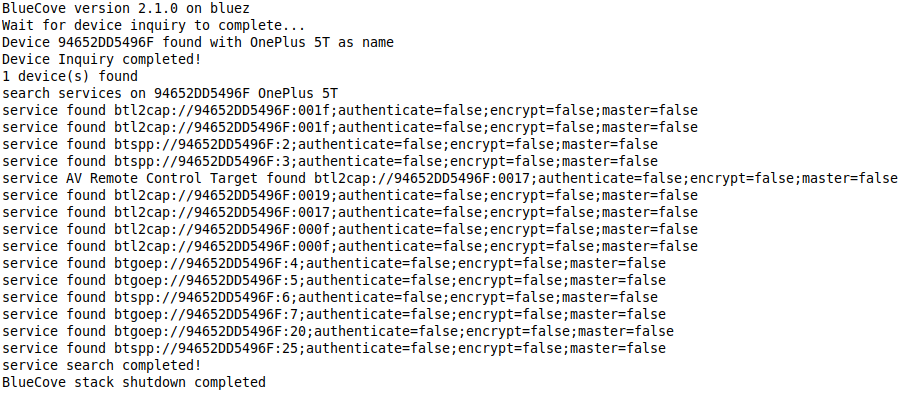
\includegraphics[scale=0.5]{imagenes/Ex7DeviceAndService.png} 
\end{flushleft}

\section{COMUNICACIÓN A TRAVÉS DE RFCOMM DE BLUETOOTH}

\subsection{Aplicación Cliente-Servidor}

Debido a problemas de compatibilidad con mi sistema operativo (Ubuntu Budgie) y las librerías, en mi ordenador da el fallo de la captura adjunta, pero he probado mi código en el ordenador de un compañero y funciona.

\begin{flushleft}
	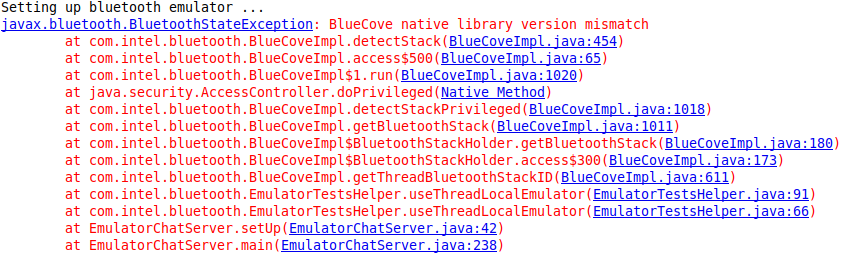
\includegraphics[scale=0.5]{imagenes/chat.png} 
\end{flushleft}

\end{document}